\documentclass[12pt]{article}

%%%%%%%%%%%%%%%%%%%%%%%%%%%%%%%%%%%%%%%%%%%%%%%%%%%%%%%%%%%%%%%%%%%%%%%%%%%%%%%%
%                           Package preset for homework
%%%%%%%%%%%%%%%%%%%%%%%%%%%%%%%%%%%%%%%%%%%%%%%%%%%%%%%%%%%%%%%%%%%%%%%%%%%%%%%%
% Miscellaneous
\usepackage[margin=1in]{geometry}
\usepackage[utf8]{inputenc}
\usepackage{indentfirst}
\usepackage{blindtext}
\usepackage{graphicx}
\usepackage{xr-hyper}
\usepackage{hyperref}
\usepackage{enumitem}
\usepackage{color}
\usepackage{float}
% Math
\usepackage{latexsym}
\usepackage{amsfonts}
\usepackage{amssymb}
\usepackage{amsmath}
\usepackage{commath}
\usepackage{amsthm}
\usepackage{bbold}
\usepackage{bm}
% Physics
\usepackage{physics}
\usepackage{siunitx}
% Code typesetting
\usepackage{listings}
% Citation
\usepackage[authoryear]{natbib}
\usepackage{appendix}
\usepackage[capitalize]{cleveref}
% Title & name
\title{Homework}
\author{Tien Vo}
\date{\today}


%%%%%%%%%%%%%%%%%%%%%%%%%%%%%%%%%%%%%%%%%%%%%%%%%%%%%%%%%%%%%%%%%%%%%%%%%%%%%%%%
%                   User-defined commands and environments
%%%%%%%%%%%%%%%%%%%%%%%%%%%%%%%%%%%%%%%%%%%%%%%%%%%%%%%%%%%%%%%%%%%%%%%%%%%%%%%%
%%% Misc
\sisetup{load-configurations=abbreviations}
\newcommand{\due}[1]{\date{Due: #1}}
\newcommand{\hint}{\textit{Hint}}
\let\oldt\t
\renewcommand{\t}[1]{\text{#1}}

%%% Bold sets & abbrv
\newcommand{\N}{\mathbb{N}}
\newcommand{\Z}{\mathbb{Z}}
\newcommand{\R}{\mathbb{R}}
\newcommand{\Q}{\mathbb{Q}}
\let\oldP\P
\renewcommand{\P}{\mathbb{P}}
\newcommand{\LL}{\mathcal{L}}
\newcommand{\FF}{\mathcal{F}}
\newcommand{\HH}{\mathcal{H}}
\newcommand{\NN}{\mathcal{N}}
\newcommand{\ZZ}{\mathcal{Z}}
\newcommand{\RN}[1]{\textup{\uppercase\expandafter{\romannumeral#1}}}
\newcommand{\ua}{\uparrow}
\newcommand{\da}{\downarrow}

%%% Unit vectors
\newcommand{\xhat}{\vb{\hat{x}}}
\newcommand{\yhat}{\vb{\hat{y}}}
\newcommand{\zhat}{\vb{\hat{z}}}
\newcommand{\nhat}{\vb{\hat{n}}}
\newcommand{\rhat}{\vb{\hat{r}}}
\newcommand{\phihat}{\bm{\hat{\phi}}}
\newcommand{\thetahat}{\bm{\hat{\theta}}}

%%% Other math stuff
\providecommand{\units}[1]{\,\ensuremath{\mathrm{#1}}\xspace}
% Set new style for problem
\newtheoremstyle{problemstyle}  % <name>
        {10pt}                   % <space above>
        {10pt}                   % <space below>
        {\normalfont}           % <body font>
        {}                      % <indent amount}
        {\bfseries\itshape}     % <theorem head font>
        {\normalfont\bfseries:} % <punctuation after theorem head>
        {.5em}                  % <space after theorem head>
        {}                      % <theorem head spec (can be left empty, 
                                % meaning `normal')>

% Set problem environment
\theoremstyle{problemstyle}
\newtheorem{problemenv}{Problem}[section]
\newenvironment{problem}[1]{%
  \renewcommand\theproblemenv{#1}%
  \problemenv
}{\endproblemenv}
% Set lemma environment
\newenvironment{lemma}[2][Lemma]{\begin{trivlist}
\item[\hskip \labelsep {\bfseries #1}\hskip \labelsep {\bfseries #2.}]}{\end{trivlist}}
% Set solution environment
\newenvironment{solution}{
    \begin{proof}[Solution]$ $\par\nobreak\ignorespaces
}{\end{proof}}
\numberwithin{equation}{problemenv}

%%% Page format
\setlength{\parindent}{0.5cm}
\setlength{\oddsidemargin}{0in}
\setlength{\textwidth}{6.5in}
\setlength{\textheight}{8.8in}
\setlength{\topmargin}{0in}
\setlength{\headheight}{18pt}

%%% Code environments
\definecolor{dkgreen}{rgb}{0,0.6,0}
\definecolor{gray}{rgb}{0.5,0.5,0.5}
\definecolor{mauve}{rgb}{0.58,0,0.82}
\lstset{frame=tb,
  language=Python,
  aboveskip=3mm,
  belowskip=3mm,
  showstringspaces=false,
  columns=flexible,
  basicstyle={\small\ttfamily},
  numbers=none,
  numberstyle=\tiny\color{gray},
  keywordstyle=\color{blue},
  commentstyle=\color{dkgreen},
  stringstyle=\color{mauve},
  breaklines=true,
  breakatwhitespace=true,
  tabsize=4
}
\lstset{
  language=Mathematica,
  numbers=left,
  numberstyle=\tiny\color{gray},
  numbersep=5pt,
  breaklines=true,
  captionpos={t},
  frame={lines},
  rulecolor=\color{black},
  framerule=0.5pt,
  columns=flexible,
  tabsize=2
}


\title{Homework 12: Phys 7310 (Fall 2021)}

\begin{document}
\maketitle
%%%%%%%%%%%%%%%%%%%%%%%%%%%%%%%%%%%%%%%%%%%%%%%%%%%%%%%%%%%%%%%%%%%%%%%%%%%%%%%
\begin{problem}{12.1}[Waves crossing a gap]
Two plane semi-infinite slabs of the same uniform, isotropic, nonpermeable,
lossless dielectric with index of refraction $n$ are parallel and separated by
an air gap ($n=1$) of width $d$. A plane electromagnetic wave of frequency
$\omega$ is incident on the gap from one of the slabs with angle of incidence
$i$. For linear polarization \textit{both} parallel to \textit{and}
perpendicular to the plane of incidence,

(a) calculate the ratio of power transmitted into the second slab to the
incident power and the ratio of reflected to incident power;

(b) for $i$ greater than the critical angle for total internal reflection,
sketch the ratio of transmitted power to incident power as a function of $d$
measured in units of wavelength in the gap (only do perpendicular polarization).
\begin{solution}
(a)
\begin{center}
    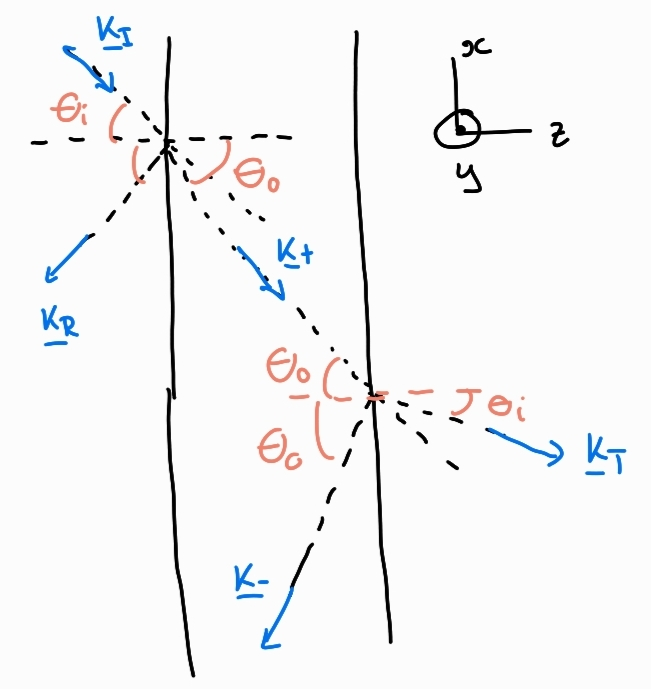
\includegraphics[width=0.5\textwidth]{hw12_p1.jpg} 
\end{center}
Given the geometry of the problem as sketched above, the incident
$I$, reflected $R$, intermediate ($\pm$ in the gap), and transmitted
$T$ wavevectors can be written as
\begin{subequations}
    \begin{align}
        \vb{k}_I&=k_1\qty(-\sin\theta_i\xhat+\cos\theta_i\zhat)\\
        \vb{k}_R&=k_1\qty(-\sin\theta_i\xhat-\cos\theta_i\zhat)\\
        \vb{k}_+&=k_2\qty(-\sin\theta_o\xhat+\cos\theta_o\zhat)\\
        \vb{k}_-&=k_2\qty(-\sin\theta_o\xhat-\cos\theta_o\zhat) \\
        \vb{k}_T&=k_3\qty(-\sin\theta_i\xhat+\cos\theta_i\zhat)\\
    \end{align} 
\end{subequations}
The boundary conditions applied at the interface between two medium 1 and 2 are
\begin{subequations}
    \begin{align}
        \qty(\epsilon_1\vb{E}_1-\epsilon_2\vb{E}_2)\vdot\zhat&=0\label{p1a:I}\\
        \qty(\vb{B}_1-\vb{B}_2)\vdot\zhat&=0\label{p1a:II}\\
        \qty(\vb{E}_1-\vb{E}_2)\times\zhat&=0\label{p1a:III}\\
        \qty(\vb{B}_1-\vb{B}_2)\times\zhat&=0\label{p1a:IV}
    \end{align} 
\end{subequations}

Now, we consider two cases
\begin{center}
\textbf{Case 1: Parallel polarization}
\end{center}

The electric field polarization is in the $(xz)$ plane. So we can write from
Faraday's law the electromagnetic fields for $z<0$ as
\begin{subequations}
    \begin{align}
        \vb{E}_I&=E_{0I}
        \qty(\cos\theta_i\xhat+\sin\theta_i\zhat)
        e^{i(\vb{k}_I\vdot\vb{x}-\omega t)}\\
        \vb{B}_I&=\sqrt{\mu\epsilon}\,\hat{\vb{k}}_I\times\vb{E}_I
        =\sqrt{\mu\epsilon}E_{0I}e^{i(\vb{k}_I\vdot\vb{x}-\omega t)}\yhat\\
        \vb{E}_R&=E_{0R}
        \qty(\cos\theta_i\xhat-\sin\theta_i\zhat)
        e^{i(\vb{k}_R\vdot\vb{x}-\omega t)}\\
        \vb{B}_R&=\sqrt{\mu\epsilon}\,\hat{\vb{k}}_R\times\vb{E}_R
        =-\sqrt{\mu\epsilon}E_{0R}e^{i(\vb{k}_R\vdot\vb{x}-\omega t)}\yhat
    \end{align} 
\end{subequations}
Similarly, for $0\leq z\leq d$,
\begin{subequations}
    \begin{align}
        \vb{E}_+&=E_{0+}
        \qty(\cos\theta_o\xhat+\sin\theta_o\zhat)
        e^{i(\vb{k}_+\vdot\vb{x}-\omega t)}\\
        \vb{B}_+&=\sqrt{\mu_0\epsilon_0}\,\hat{\vb{k}}_+\times\vb{E}_+
        =\sqrt{\mu_0\epsilon_0}E_{0+}e^{i(\vb{k}_+\vdot\vb{x}-\omega t)}\yhat\\
        \vb{E}_-&=E_{0-}
        \qty(\cos\theta_o\xhat-\sin\theta_o\zhat)
        e^{i(\vb{k}_-\vdot\vb{x}-\omega t)}\\
        \vb{B}_-&=\sqrt{\mu_0\epsilon_0}\,\hat{\vb{k}}_-\times\vb{E}_-
        =-\sqrt{\mu_0\epsilon_0}E_{0-}e^{i(\vb{k}_-\vdot\vb{x}-\omega t)}\yhat
    \end{align} 
\end{subequations}
and for $z>d$,
\begin{subequations}
    \begin{align}
        \vb{E}_T&=E_{0T}
        \qty(\cos\theta_i\xhat+\sin\theta_i\zhat)
        e^{i(\vb{k}_T\vdot\vb{x}-\omega t)}\\
        \vb{B}_T&=\sqrt{\mu\epsilon}\,\hat{\vb{k}}_T\times\vb{E}_T
        =\sqrt{\mu\epsilon}E_{0T}e^{i(\vb{k}_T\vdot\vb{x}-\omega t)}\yhat
    \end{align} 
\end{subequations}
Applying the boundary conditions at $z=0$, we first get from \eqref{p1a:I},
\begin{equation}\label{p1a:1}
    \epsilon\sin\theta_i(E_{0I}-E_{0R})
    =\epsilon_0\sin\theta_0\qty(E_{0+}-E_{0-})
    \Rightarrow E_{0+}-E_{0-}=n(E_{0I}-E_{0R})
\end{equation}
and \eqref{p1a:III},
\begin{equation}\label{p1a:2}
    \cos\theta_i(E_{0I}+E_{0R})=\cos\theta_o\qty(E_{0+}+E_{0-})
    \Rightarrow E_{0+}+E_{0-}=\frac{\cos\theta_i}{\cos\theta_o}(E_{0I}+E_{0R})
\end{equation}

Similarly, at $z=d$, we attain from \eqref{p1a:I},
\begin{align}\label{p1a:3}
    &&\epsilon_0\sin\theta_i
    \qty(E_{0+}e^{ik_2d\cos\theta_o}-E_{0-}e^{-ik_2d\cos\theta_o}) 
    &=\epsilon\sin\theta_i E_{0T} e^{ik_3d\cos\theta_i}\notag\\
    &\Rightarrow&
    E_{0+}e^{ik_2d\cos\theta_o}-E_{0-}e^{-ik_2d\cos\theta_o}
    &=nE_{0T}e^{ik_3d\cos\theta_i}
\end{align}
and from \eqref{p1a:III},
\begin{align}\label{p1a:4}
    &&\cos\theta_o
    \qty(E_{0+}e^{ik_2d\cos\theta_o}+E_{0-}e^{-ik_2d\cos\theta_o}) 
    &=\cos\theta_i E_{0T}e^{ik_3d\cos\theta_i}\notag\\
    &\Rightarrow&
    E_{0+}e^{ik_2d\cos\theta_o}+E_{0-}e^{-ik_2d\cos\theta_o}
    &=\frac{\cos\theta_i}{\cos\theta_o}E_{0T}e^{ik_3d\cos\theta_i}
\end{align}

Solving the system \eqref{p1a:1}, \eqref{p1a:2}, \eqref{p1a:3}, \eqref{p1a:4}
with Mathematica, we get
\begin{subequations}
    \begin{align}
        E_{0+}
        &=E_{0T}\frac{\cos\theta_i+n\cos\theta_o}{2\cos\theta_o}e^{ik_3d\cos\theta_i}e^{-ik_2d\cos\theta_o}\\
        E_{0-}
        &=E_{0T}\frac{\cos\theta_i -n\cos\theta_o}{2\cos\theta_o}
        e^{ik_3d\cos\theta_i}e^{-ik_2d\cos\theta_o}
    \end{align} 
\end{subequations}
From \eqref{p1a:1} and \eqref{p1a:2}, we can write
\begin{align}
    &&2E_{0I}&=\frac1n\qty(E_{0+}-E_{0-})+\frac{\cos\theta_o}{\cos\theta_i}\qty(E_{0+}+E_{0-})\notag\\
    &&&=\frac{\cos\theta_i+n\cos\theta_o}{n\cos\theta_i}E_{0+}
    -\frac{\cos\theta_i-n\cos\theta_o}{n\cos\theta_i}E_{0-}\notag\\
    &\Rightarrow&
    4n\cos\theta_i\cos\theta_o\frac{E_{0I}}{E_{0T}}
    &=e^{ik_3d\cos\theta_i}\qty[(\cos\theta_i+n\cos\theta_o)^2e^{-ik_2d\cos\theta_o}-(\cos\theta_i-n\cos\theta_o)^2e^{ik_2d\cos\theta_o}]\notag\\
    &\Rightarrow&
    4n\cos\theta_i\cos\theta_o\abs{\frac{E_{0I}}{E_{0T}}}
    &=4\abs{(\cos^2\theta_i+n^2\cos^2\theta_o)\sin\alpha
    +2i\cos\theta_i\cos\theta_o\cos\alpha}\tag{$\alpha=k_2d\cos\theta_o$}\\
    &\Rightarrow&
    n^2\cos^2\theta_i\cos^2\theta_o\frac1T
    &=\qty(\cos^2\theta_i+n^2\cos^2\theta_o)^2\sin^2\alpha
    +4\cos^2\theta_i\cos^2\theta_o\cos^2\alpha
\end{align}
Thus, the transmission coefficient is
\begin{equation}
    T=\frac{n^2\cos^2\theta_i\cos^2\theta_o}{(\cos^2\theta_i+n^2\cos^2\theta_o)^2\sin^2\alpha+4\cos^2\theta_i\cos^2\theta_o\cos^2\alpha} 
\end{equation}
where $\alpha=(\omega d/c)\cos\theta_o$ and
$\cos\theta_o=\sqrt{1-n^2\sin^2\theta_i}$ from Snell's Law. The reflection
coefficient is just trivially $R=1-T$, by energy conservation.

\begin{center}
\textbf{Case 2: Perpendicular polarization}
\end{center}
Similar to the first case, we can write the fields for $z<0$ as
\begin{subequations}
    \begin{align}
        \vb{E}_I&=E_{0I}e^{i(\vb{k}_I\vdot\vb{x}-\omega t)}\yhat\\
        \vb{B}_I&=\sqrt{\mu\epsilon}E_{0I}(-\cos\theta_i\xhat-\sin\theta_i\zhat)e^{i(\vb{k}_I\vdot\vb{x}-\omega
        t)}\\
        \vb{E}_R&=E_{0R}e^{i(\vb{k}_R\vdot\vb{x}-\omega t)}\yhat\\
        \vb{B}_R&=\sqrt{\mu\epsilon}E_{0R}(\cos\theta_i\xhat-\sin\theta_i\zhat)e^{i(\vb{k}_R\vdot\vb{x}-\omega
        t)}
    \end{align} 
\end{subequations}
For $0\leq z\leq d$,
\begin{subequations}
    \begin{align}
        \vb{E}_+&=E_{0+}e^{i(\vb{k}_+\vdot\vb{x}-\omega t)}\yhat\\
        \vb{B}_+&=\sqrt{\mu_0\epsilon_0}E_{0+}(-\cos\theta_o\xhat-\sin\theta_o\zhat)e^{i(\vb{k}_+\vdot\vb{x}-\omega
        t)}\\
        \vb{E}_-&=E_{0-}e^{i(\vb{k}_-\vdot\vb{x}-\omega t)}\yhat\\
        \vb{B}_-&=\sqrt{\mu_0\epsilon_0}E_{0-}(\cos\theta_o\xhat-\sin\theta_o\zhat)e^{i(\vb{k}_-\vdot\vb{x}-\omega
        t)}
    \end{align} 
\end{subequations}
For $z>d$,
\begin{subequations}
    \begin{align}
        \vb{E}_T&=E_{0T}e^{i(\vb{k}_T\vdot\vb{x}-\omega t)}\yhat\\
        \vb{B}_T&=\sqrt{\mu\epsilon}E_{0T}(-\cos\theta_i\xhat-\sin\theta_i\zhat)e^{i(\vb{k}_T\vdot\vb{x}-\omega
        t)}
    \end{align} 
\end{subequations}

Applying the boundary conditions \eqref{p1a:II} at $z=0$, we get
\begin{align}\label{p1a:5}
    \sqrt{\mu\epsilon}\sin\theta_i(-E_{0I}-E_{0R})=\sqrt{\mu_0\epsilon_0}\sin\theta_o\qty(-E_{0+}-E_{0-})\Rightarrow
    E_{0I}+E_{0R}=E_{0+}+E_{0-}
\end{align}
and at $z=d$, we get
\begin{align}\label{p1a:6}
    &&\sqrt{\mu_0\epsilon_0}\sin\theta_o(-E_{0+}e^{ik_2d\cos\theta_o}-E_{0-}e^{-ik_2d\cos\theta_o})
    &=\sqrt{\mu\epsilon}\sin\theta_iE_{0T}e^{ik_3d\cos\theta_i}\\
    &\Rightarrow&
    E_{0+}e^{ik_2d\cos\theta_o}+E_{0-}e^{-ik_2d\cos\theta_o}
    &=E_{0T}e^{ik_3d\cos\theta_i}
\end{align}

Applying \eqref{p1a:IV} at $z=0$, we get
\begin{equation}\label{p1a:7}
    \sqrt{\mu\epsilon}\cos\theta_i(-E_{0I}+E_{0R})
    =\sqrt{\mu_0\epsilon_0}\cos\theta_o\qty(-E_{0+}+E_{0-})
    \Rightarrow
    E_{0+}-E_{0-}=\frac{n\cos\theta_i}{\cos\theta_o}\qty(E_{0I}-E_{0R})
\end{equation}
and at $z=d$, we get
\begin{align}\label{p1a:8}
    &&\sqrt{\mu_0\epsilon_0}\cos\theta_o\qty(-E_{0+}e^{ik_2d\cos\theta_o}+E_{0-}e^{-ik_2d\cos\theta_o})
    &=-\sqrt{\mu\epsilon}\cos\theta_iE_{0T}e^{ik_3d\cos\theta_i}\notag\\
    &\Rightarrow&
    E_{0+}e^{ik_2d\cos\theta_o}-E_{0-}e^{-ik_2d\cos\theta_o}
    &=\frac{n\cos\theta_i}{\cos\theta_o}E_{0T}e^{ik_3d\cos\theta_i}
\end{align}

Using Mathematica to solve \eqref{p1a:5}, \eqref{p1a:6}, \eqref{p1a:7}, and
\eqref{p1a:8}, we get
\begin{subequations}
    \begin{align}
        E_{0+}&=\frac12E_{0T}\qty(1+\frac{n\cos\theta_i}{\cos\theta_o})e^{ik_3d\cos\theta_i}e^{-ik_2d\cos\theta_o}\\ 
        E_{0-}&=\frac12E_{0T}\qty(1-\frac{n\cos\theta_i}{\cos\theta_o})
        e^{ik_3d\cos\theta_i}e^{ik_2\cos\theta_o}
    \end{align} 
\end{subequations}
Then we can write from \eqref{p1a:5} and \eqref{p1a:7} that
\begin{align}
    &&2E_{0I}&=\frac{\cos\theta_o+n\cos\theta_i}{n\cos\theta_i}E_{0+}
    -\frac{\cos\theta_o-n\cos\theta_i}{n\cos\theta_i}E_{0-}\notag\\
    &\Rightarrow&
    4n\cos\theta_i\cos\theta_o\frac{E_{0I}}{E_{0T}}
    &=e^{ik_3d\cos\theta_i}\qty[(\cos\theta_o+n\cos\theta_i)^2e^{-i\alpha}-(\cos\theta_o-n\cos\theta_i)^2e^{i\alpha}]\notag\\
    &\Rightarrow&
    4n\cos\theta_i\cos\theta_o\abs{\frac{E_{0I}}{E_{0T}}}&=
\abs{4n\cos\theta_i\cos\theta_o\cos\alpha-2i(n^2\cos^2\theta_i+\cos^2\theta_o)\sin\alpha}\notag\\
    &\Rightarrow&
    4n^2\cos^2\theta_i\cos^2\theta_o\frac1T
    &=4n^2\cos^2\theta_i\cos^2\theta_o\cos^2\alpha
    +(n^2\cos^2\theta_i+\cos^2\theta_o)^2\sin^2\alpha
\end{align}
Then the transmission coefficient is
\begin{equation}\label{p1a:T}
    T=\frac{4n^2\cos^2\theta_i\cos^2\theta_o}{4n^2\cos^2\theta_i\cos^2\theta_o\cos^2\alpha+(n^2\cos^2\theta_i+\cos^2\theta_o)^2\sin^2\alpha} 
\end{equation}
and the reflection coefficient is simplify $R=1-T$, where $\cos\theta_o$ and
$\alpha$ retain the same definitions as in the first case.

(b) If $\theta_i\geq \theta_c$ such that $n\sin\theta_c=1$, then
$1<n^2\sin^2\theta_i$ and $\alpha=(\omega
d/c)\sqrt{1-n^2\sin^2\theta_i}=i(\omega d/c)\sqrt{n^2\sin^2\theta_i-1}=i\psi$.
It also follows that $\cos\alpha=\cosh\psi$ and $\sin\alpha=i\sinh\psi$. From
\eqref{p1a:T}, the transmission coefficient for angles above the critical angle
$\theta_c$ is
\begin{equation}
    T=\frac{4n^2\cos^2\theta_i\cos^2\theta_o}{4n^2\cos^2\theta_i\cos^2\theta_o\cosh^2\psi-(n^2\cos^2\theta_i+\cos^2\theta_o)^2\sinh^2\psi}
\end{equation}
where $\psi=(\omega
d/c)\sqrt{n^2\sin^2\theta_i-1}=2\pi\sqrt{n^2\sin^2\theta_i-1}(d/\lambda)$. In 
the following, we plot the transmission coefficient for water $(n=1.3)$ and
$\theta_i=60^\circ$
\begin{center}
    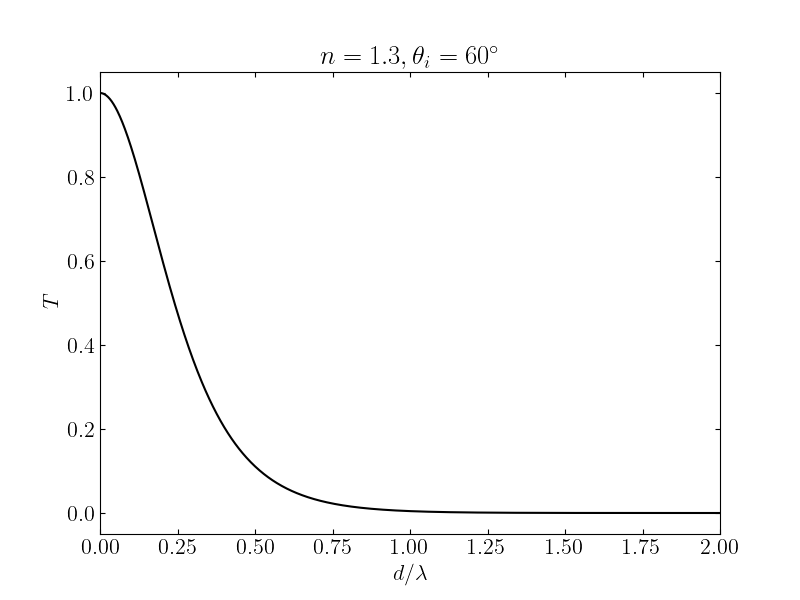
\includegraphics[width=0.8\textwidth]{p1.png} 
\end{center}
\end{solution}
\end{problem}
%%%%%%%%%%%%%%%%%%%%%%%%%%%%%%%%%%%%%%%%%%%%%%%%%%%%%%%%%%%%%%%%%%%%%%%%%%%%%%%    
%%%%%%%%%%%%%%%%%%%%%%%%%%%%%%%%%%%%%%%%%%%%%%%%%%%%%%%%%%%%%%%%%%%%%%%%%%%%%%%
\begin{problem}{12.2}[Wave entering a conductor]
A plane wave of frequency $\omega$ is incident normally from vacuum on a
semi-infinite slab of material with a \textit{complex} index of refraction
$n(\omega)$ [$n^2(\omega)=\epsilon(\omega)/\epsilon_0$].

(a) Show that the ratio of reflected power to incident power is
\begin{equation}
    R=\abs{\frac{1-n(\omega)}{1+n(\omega)}}^2 
\end{equation}
while the ratio of power transmitted into the medium to the incident power is 
\begin{equation}
    T=\frac{4\Re n(\omega)}{\abs{1+n(\omega)}^2} 
\end{equation}

(b) Evaluate $\Re\qty[i\omega(\vb{E}\vdot\vb{D}^\ast-\vb{B}\vdot\vb{H}^\ast)/2]$
as a function of $(x,y,z)$. Show that this rate of change of energy per unit
volume accounts for the relative transmitted power $T$. Compare the quantity
mentioned to $T\vb{S}_i$ (the fraction of the incident flux that is transmitted)
where $\vb{S}_i$ is the real, time-averaged Poynting flux
$(1/2)\Re\qty(\vb{E}\times\vb{H}^\ast)$.

(c) For a conductor, with $n^2=1+i(\sigma/\omega\epsilon_0)$, $\sigma$ real,
write out the results of parts (a) and (b) in the limit
$\epsilon_0\omega\ll\sigma$. Express your answer in terms of
$\delta=\sqrt{2/\mu\sigma\omega}$ as much as
possible. Calculate $(1/2)\Re(\vb{J}^\ast\vdot\vb{E})$ and compare with the
results of part (b). Do both enter the complex form of Poynting's theorem?
\begin{solution}
    (a) The reflection coefficient follows simply from (7.42, Jackson) that
\begin{equation}
    R=\abs{\frac{E_{0R}}{E_{0I}}}^2
    =\abs{\frac{1-n}{1+n}}^2
\end{equation}
since the derivations leading to that equation does not depend on the complexity
of $n$. Now, we write $n=\Re(n)+i\Im(n)$ and calculate
\begin{align}
    T&=1-R\notag\\
     &=1-\qty(\frac{1-n}{1+n})\qty(\frac{1-n}{1+n})^\ast\notag\\
     &=\frac{(1+\Re(n)+i\Im(n))(1+\Re(n)-i\Im(n))-(1-\Re(n)-i\Im(n))(1-\Re(n)+i\Im(n))}{\abs{1+n}^2}\notag\\
     &=\frac{4\Re(n)}{\abs{1+n}^2}
\end{align}
where we have simplified the last step with Mathematica.

(b) First, the electric field of a wave propagating along the $z$ direction is
\begin{equation}
    \vb{E}=\vb{E}_0e^{i(kz-\omega t)} 
    =\vb{E}_0e^{-\Im(k)z}e^{i(\Re(k)z-\omega t)}
\end{equation}
where $\vb{E}_0$ is in the $(xy)$ plane. It then folows that
\begin{equation}
    \abs{\vb{k}\times\vb{E}}^2
    =\abs{\vb{k}\times\vb{E}_0}e^{-2\Im(k)z}
    =\abs{k}^2E_0^2e^{-2\Im(k)z}
\end{equation}
So the rate of change in energy density is
\begin{align}
    C
    &=\Re\frac{i\omega}{2}\qty(\vb{E}\vdot\vb{D}^\ast-\vb{B}\vdot\vb{H}^\ast)\notag\\
    &=\Re\frac{i\omega}{2}\qty(\epsilon^\ast\abs{E}^2-\frac1{\mu}\abs{B}^2)\notag\\
    &=\Re\frac{i\omega}{2}\qty[\epsilon^\ast
    E_0^2e^{-2\Im(k)z}-\frac1{\mu\omega^2}\abs{k}^2E_0^2e^{-2\Im(k)z}]\notag\\
    &=\Re\frac{i\omega}{2}\qty(\frac{\epsilon^\ast}{\epsilon_0}-\frac{\abs{k}^2}{\epsilon_0\mu\omega^2})\epsilon_0E_0^2e^{-2\Im(k)z}\notag\\
    &=\Re\frac{i\omega}{2}\epsilon_0E_0^2e^{-2\Im(k)z}\qty[(n^\ast)^2-\abs{n}^2]\notag\\
    &=\frac{\omega}{2}\epsilon_0E_0^2e^{-2\Im(k)z}\Re\qty[2(\Re(n)-i\Im(n))\Im(n)]\notag\\
    &=\omega\epsilon_0E_0^2e^{-2\Im(k)z}\Re(n)\Im(n)
\end{align}

By definition, the incident Poynting flux is
\begin{align}
    S_i&=\frac12\abs{\Re\qty{\vb{E}_i\times\vb{H}_i}}\notag\\
    &=\frac1{2\mu_0}\abs{\Re\qty{\vb{E}_i\times\vb{B}_i^\ast}}\notag\\
    &=\frac12\sqrt{\frac{\epsilon_0}{\mu_0}}\abs{\Re\qty{\abs{E_i}^2\hat{\vb{k}}_i}}\notag\\
    &=\frac12\sqrt{\frac{\epsilon_0}{\mu_0}}\abs{E_i}^2
\end{align}
We can also calculate the transmitted Poynting flux (energy flux) from the rate
of change in energy density by integrating over the half-infinite medium
\begin{align}
    S_t
    &=\int_0^\infty dzC\notag\\
    &=\int_0^\infty
    dz\omega\epsilon_0E_0^2\Re(n)\Im(n)e^{-2\omega\Im(n)z/c}\notag\\
    &=\frac{c}{2\omega\Im(n)}\omega\epsilon_0E_0^2\Re(n)\Im(n)\notag\\
    &=\frac12\sqrt{\frac{\epsilon_0}{\mu_0}}\abs{E_t}^2\Re(n)
\end{align}
Then the ratio between these fluxes is exactly the same as the transmission
coefficient
\begin{equation}
    \frac{S_t}{S_i}=\Re(n)\abs{\frac{E_t}{E_i}}^2=T 
\end{equation}
Thus, $S_t=TS_i$. The rate of change in energy density accounts for the
transmitted energy flux.

(c) First, $n^2=1+i(\sigma/\omega\epsilon_0)=1+i/x\approx
i/x=(1/x)e^{i\pi/2}$ if $x\ll 1$. Then we can write
\begin{equation}
    n=\frac1{\sqrt{x}}e^{i\pi/4} 
\end{equation}
From part (a), the reflection coefficient is
\begin{align}
    R&=\abs{\frac{1-n}{1+n}}^2\notag\\
     &=\abs{1+\frac2{\sqrt{x}e^{3i\pi/4}-1}}^2\notag\\
     &\approx\abs{-1-2\sqrt{x}e^{3i\pi/4}}^2\notag\\
     &=\abs{-1-\sqrt{2x}(-1+i)}^2\notag\\
     &=(\sqrt{2x}-1)^2+2x\notag\\
     &\approx1-2\sqrt{2x}\notag\\
     &=1-2\frac{\delta\omega}{c}
\end{align}
where $\delta=\sqrt{2/\mu\sigma\omega}$. Similarly, the transmission coefficient
is
\begin{align}
    T&=\frac{4\Re(n)}{\abs{1+n}^2}\notag\\
     &=\frac{4/\sqrt{2x}}{1+(1/\sqrt{x})e^{i\pi/4}}^2\notag\\
     &=\frac{4/\sqrt{2x}}{(1+1/\sqrt{2x})^2+1/2x}\notag\\
     &\approx2\sqrt{2x}\notag\\
     &=2\frac{\delta\omega}{c}
\end{align}
which guarantees that $R+T=1$. From part (b), the rate of change in energy
density is
\begin{align}
    C&=\omega\epsilon_0E_0^2e^{-2\omega \Im(n)z/c}\Re(n)\Im(n) \notag\\
     &=\omega\epsilon_0E_0^2e^{-2\omega z/c\sqrt{2x}}\frac1{2x}\notag\\
     &=\frac12\sigma E_0^2e^{-2z/\delta}\notag\\
     &=\frac{1}{\mu\omega\delta^2}e^{-2z/\delta}E_0^2
\end{align}
Now, we calculate with the generalized Ohm's Law,
$\vb{J}=\sigma\vb{E}$, to confirm that
\begin{align}
    \frac12\Re\qty{\vb{J}^\ast\vdot\vb{E}} 
    =\frac{\sigma}{2}\Re\qty{\vb{E}^\ast\vdot\vb{E}}
    =\frac{\sigma}{2}E_0^2e^{-2\Im(k)z}
    =C
\end{align}
Since these are the same, the energy transmitted must be lost to Joule heating.
\end{solution}
\end{problem}
%%%%%%%%%%%%%%%%%%%%%%%%%%%%%%%%%%%%%%%%%%%%%%%%%%%%%%%%%%%%%%%%%%%%%%%%%%%%%%%
%%%%%%%%%%%%%%%%%%%%%%%%%%%%%%%%%%%%%%%%%%%%%%%%%%%%%%%%%%%%%%%%%%%%%%%%%%%%%%%
\begin{problem}{12.3}[Wave propagation through a stack of layers]
A monochromatic plane wave of frequency $\omega$ is incident normally on a stack
of layers of various thicknesses $t_j$ and lossless indices of refraction $n_j$.
Inside the stack, the wave has both forward and backward moving components. The
change in the wave through any interface and also from one side of a layer to
the other can be described by means of $2\times 2$ transfer matrices. If the
electric field is written as
\begin{equation}
    E=E_+e^{ikx}+E_-e^{-ikx} 
\end{equation}
in each layer, the transfer matrix equation $E'=TE$ is explicitly
\begin{equation}
    \mqty(E_+'\\E_-')=\mqty(t_{11}&t_{12}\\t_{21}&t_{22})\mqty(E_+\\E_-)
\end{equation}

(a) Show that the transfer matrix for propagation inside, but across, a layer of
index of refraction $n_j$ and thickness $t_j$ is
\begin{equation}
    T_\text{layer}(n_j,t_j)=\mqty(e^{ik_jt_j}&0\\0&e^{-ik_jt_j})=I\cos\qty(k_jt_j)+i\sigma_3\sin\qty(k_jt_j) 
\end{equation}
where $k_j=n_j\omega/c$, $I$ is the unit matrix, and $\sigma_k$ are the Pauli
spin matrices of quantum mechanics. Show that the inverse matrix is $T^\ast$.

(b) Show that the transfer matrix to cross an interface from $n_1(x<x_0)$ to
$n_2(x>x_0)$ is
\begin{equation}
    T_\text{interface}(2,1)=\frac12\mqty(n+1&-(n-1)\\-(n-1)&n+1)=I\frac{n+1}{2}-\sigma_1\frac{n-1}{2} 
\end{equation}
where $n=n_1/n_2$.

(c) Show that for a complete stack, the incident, reflected, and transmitted
waves are related by
\begin{equation}
    E_\text{trans}=\frac{\det(T)}{t_{22}}E_\text{inc},\qquad
    E_\text{refl}=-\frac{t_{21}}{t_{22}}E_\text{inc}
\end{equation}
where $t_{ij}$ are the elements of $T$, the product of the forward-going
transfer matrices, including from the material filling space on the incident
side into the first layer and from the last layer into the medium filling the
space on the transmitted side.
\begin{solution}
(a) Given the electric field in the layer $n_j$
\begin{equation}
    E(x)=E_+e^{ik_jx}+E_-e^{-ik_jx} 
\end{equation}
By a translation $x\mapsto x+t_j$, the electric field becomes
\begin{equation}
    E(x+t_j)=E_+e^{ik_j(x+t_j)}+E_-e^{-ik_j(x+t_j)}
    =E_+e^{ik_jt_j}e^{ik_jx}+E_-e^{-ik_jt_j}e^{-ik_jx}
\end{equation}
Thus, the transferred amplitude of the forward and backward electric field is
$E_\pm'$ where
\begin{equation}
    E_\pm'=E_\pm e^{\pm ik_jt_j}
\end{equation}
or
\begin{equation}
    \mqty(E_+'\\E_-')=\mqty(e^{ik_jt_j}&0\\0&e^{-ik_jt_j})\mqty(E_+\\E_-)
\end{equation}
Thus,
\begin{align}
    T_\text{layer}
    &=\mqty(e^{ik_jt_j}&0\\0&e^{-ik_jt_j})\notag\\
    &=\mqty(\cos(k_jt_j)+i\sin(k_jt_j)&0\\0&\cos(k_jt_j)-i\sin(k_jt_j))\notag\\
    &=I\cos(k_jt_j)+i\mqty(1&0\\0&-1)\sin(k_jt_j)\notag\\
    &=I\cos(k_jt_j)+i\sigma_3\sin(k_jt_j)
\end{align}
Since $T_\text{layer}$ is diagonal, the inverse of $T$ is
\begin{align}
    T^{-1}=\mqty(1/e^{ik_jt_j}&0\\0&1/e^{-ik_jt_j})
    =\mqty(e^{-ik_jt_j}&0\\0&e^{ik_jt_j})
    =T^\ast
\end{align}

(b) At the boundary, the electric field and magnetic field are continuous. Thus,
it follows that
\begin{equation}
    E_++E_-=E_+'+E_-' 
    \qquad\text{and}\qquad
    n_1(E_+-E_-)=n_2(E_+'-E_-')
\end{equation}
Solving this system of equations, we can write
\begin{subequations}
   \begin{align}
       E_+'&=\frac12\qty[(1+n)E_++(1-n)E_-]\\
       E_-'&=\frac12\qty[(1-n)E_++(1+n)E_-]
   \end{align} 
\end{subequations}
or,
\begin{equation}
    \mqty(E_+'\\E_-')=\frac12\mqty(1+n&1-n\\1-n&1+n)\mqty(E_+\\E_-)
\end{equation}
So the transfer matrix is
\begin{align}
    T_\text{interface}
    &=\frac12\mqty(1+n&1-n\\1-n&1+n)\notag\\
    &=\frac12\mqty(1+n&0\\0&1+n)+\frac12\mqty(0&1-n\\1-n&0)\notag\\
    &=I\frac{n+1}{2}+\sigma_1\frac{1-n}{2}
\end{align}

(c) At the last layer, there is no backward-propagating wave, so the transfer
equation is
\begin{equation}
    \mqty(E_{0T}\\0)=\mqty(t_{11}&t_{12}\\t_{21}&t_{22})\mqty(E_{0I}\\E_{0R}) 
\end{equation}
which equates to
\begin{equation}
    E_{0T}=t_{11}E_{0I}+t_{12}E_{0R} 
    \qquad\text{and}\qquad
    t_{21}E_{0I}+t_{22}E_{0R}
\end{equation}
From the latter, we can write
\begin{equation}
    \frac{E_{0R}}{E_{0I}}=-\frac{t_{21}}{t_{22}} 
\end{equation}
and from the latter,
\begin{equation}
    \frac{E_{0T}}{E_{0I}}=t_{11}+t_{12}\frac{E_{0R}}{E_{0I}} 
    =\frac{t_{11}t_{22}-t_{12}t_{21}}{t_{22}}
    =\frac{\det\qty(T)}{t_{22}}
\end{equation}
\end{solution}
\end{problem}
%%%%%%%%%%%%%%%%%%%%%%%%%%%%%%%%%%%%%%%%%%%%%%%%%%%%%%%%%%%%%%%%%%%%%%%%%%%%%%%
\end{document}
